\documentclass[11pt]{book}

\input conditional.tex
%\def\debugmode{}

% include figures
\usepackage{epsfig,wrapfig}

% prefer PDF to PNG
\DeclareGraphicsExtensions{%
  .pdf, .png}

\graphicspath{{preface/}{intro/}{finite-volume/}{advection/}{burgers/}{diffusion/}{Euler/}{incompressible/}{multigrid/}{multiphysics/}{low_mach/}{radiation/}{pyro/}}

% AMS symbols
\usepackage{amsmath,amssymb}

% cancel
\usepackage{cancel}

% Palatino font (and math symbols) -- looks nicer than the standard
% LaTeX font
\usepackage{mathpazo}
%\usepackage{helvet}

% URLs (special font for monospace)
%\usepackage{inconsolata}
%\usepackage[T1]{fontenc}


% margins and paper size -- this needs to come before fncychap
% see http://stackoverflow.com/questions/3729099/latex-paper-size
\usepackage[top=0.75in,
            bottom=0.75in,
            inner=0.65in,
            outer=0.65in]{geometry}
\geometry{papersize={7in,10in}}

% crop marks (for printing)
%\usepackage[
%  noinfo,
%  cam,
%  cross,                % crosses as marks
%  width=7.25in,         % the width of the galley
%  height=10.25in,        % the height of the galley
%  center                % actual page is centered on the galley
%]{crop}


% this needs to be done before the fncychap style, since that will
% redo the chapter stuff
\usepackage{sectsty}
\allsectionsfont{\sffamily}


% chapter title styles
%\usepackage[Bjornstrup]{fncychap}
%\ChNumVar{\fontsize{76}{80}\usefont{OT1}{pzc}{m}{n}\selectfont}
%\ChTitleVar{\raggedleft\Large\sffamily\bfseries}

\usepackage[PetersLenny]{fncychap}
\ChNameVar{\fontsize{16}{18}\usefont{OT1}{phv}{m}{n}\selectfont}
\ChNumVar{\fontsize{60}{62}\usefont{OT1}{ptm}{m}{n}\selectfont}
\ChTitleVar{\Huge\bfseries\sffamily}
\ChRuleWidth{1pt}

% part page style
% see http://tex.stackexchange.com/questions/6609/problems-with-part-labels-using-titlesec
\usepackage{titlesec}

\titleformat{\part}[display]
   {\bfseries\sffamily\Huge\filcenter}
   {{\partname{}} \thepart}
   {0em}
   {\hrule}




% hyperlinks -- load after fncychap
\usepackage{hyperref}
\usepackage[hyperpageref]{backref}
\renewcommand*{\backref}[1]{}% for backref < 1.33 necessary
\renewcommand*{\backrefalt}[4]{%
\ifcase #1 %
  No citations.%
\or
  (Cited on page #2)%
\else
  (Cited on pages #2)%
\fi
}

% back references


% color package
\usepackage{xcolor}
\definecolor{mygray}{gray}{0.5}


% custom hrule for title page
\newcommand{\HRule}{\rule{\linewidth}{0.125mm}}

\newcommand{\pyro}{{\sf pyro}}
\newcommand{\git}{{\tt git}}

\newcommand{\ddx}[1]{{\frac{{\partial#1}}{\partial x}}}

\usepackage{xfrac}
%% \newcommand{\sfrac}[2]{\mathchoice
%%   {\kern0em\raise.5ex\hbox{\the\scriptfont0 #1}\kern-.15em/
%%    \kern-.15em\lower.25ex\hbox{\the\scriptfont0 #2}}
%%   {\kern0em\raise.5ex\hbox{\the\scriptfont0 #1}\kern-.15em/
%%    \kern-.15em\lower.25ex\hbox{\the\scriptfont0 #2}}
%%   {\kern0em\raise.5ex\hbox{\the\scriptscriptfont0 #1}\kern-.2em/
%%    \kern-.15em\lower.25ex\hbox{\the\scriptscriptfont0 #2}}
%%   {#1\!/#2}}


\newcommand{\myhalf}{\sfrac{1}{2}}
\newcommand{\mythreehalf}{\sfrac{3}{2}}
\newcommand{\mydxh}{\sfrac{\Delta x}{2}}
\newcommand{\mydth}{\sfrac{\Delta t}{2}}


% footer
%% \usepackage{fancyhdr}
%% \pagestyle{fancy}
%% \fancyfoot[LO,LE]{\footnotesize \sffamily \color{mygray} M.\ Zingale---Notes on the Euler equations}
%% \fancyfoot[RO,RE]{\footnotesize \sffamily \color{mygray} (\today)}
%% \fancyfoot[CO,CE]{\thepage}
%% \fancyhead{}
%% \renewcommand{\headrulewidth}{0.0pt}
%% \renewcommand{\footrulewidth}{0.0pt}



% don't make the chapter/section headings uppercase.  See the fancyhdr
% documentation (section 9)
\usepackage{fancyhdr}
\renewcommand{\chaptermark}[1]{%
\markboth{\chaptername
\ \thechapter.\ #1}{}}

\renewcommand{\sectionmark}[1]{\markright{\thesection---#1}}


% don't put a header on blank pages, see
% http://www.latex-community.org/forum/viewtopic.php?f=4&p=51559
% change ``plain'' to ``empty'' to eliminate the page number
\makeatletter
\renewcommand*\cleardoublepage{\clearpage\if@twoside
\ifodd\c@page\else
\hbox{}
\thispagestyle{empty}
\newpage
\if@twocolumn\hbox{}\newpage\fi\fi\fi}
\makeatother




% skip a bit of space between paragraphs, to enhance readability
\usepackage{parskip}


% captions
\usepackage{caption}
\renewcommand{\captionfont}{\footnotesize}
\renewcommand{\captionlabelfont}{\footnotesize}
\setlength{\captionmargin}{3em}


%-----------------------------------------------------------------------------
% define a new environment for exercises
%\newcounter{exercise}    % simple way -- no TOC list
% toclot allows us to make a list of exercises
% the new environment stuff came from http://www.dickimaw-books.com/latex/novices/html/newenv.html
\usepackage{tocloft}
\newcommand{\listexercisename}{List of Exercises}

% the [chapter] argumenet here means that we reset the numbers each chapter
% exc is the short name we give to this new list
\newlistof[chapter]{exercise}{exc}{\listexercisename}
\usepackage{changepage}   % used to adjust the margins within the environment

% environment name, with optional argument for display in the list of
% exercises
\newenvironment{exercise}[1][]
{% begin code
  %
  % this indents our text from the left and right
  \begin{adjustwidth}{1.0cm}{1.0cm}
  %
  % this skips a line before
  \par\vspace{\baselineskip}\noindent
  %
  % this increments our counter
  \refstepcounter{exercise}%
  %
  % this displays the exercise number and starts italics
  \textbf{\sffamily Exercise \theexercise:}\ \begin{itshape}%
  %
  % this adds an entry to our custom List of Exercises
  \addcontentsline{exc}{exercise}{\protect\numberline{\theexercise}~~ #1}
}%
{% end code -- this is done at the end of the environment
  %
  % stop the italics
  \end{itshape}%
  %
  % this stops our custom margins
  \end{adjustwidth}%
  %
  % this skips a line at the end
  \vspace{\baselineskip}\ignorespacesafterend
}

% this makes the List of Exercises have a line break before each chapter,
% just like in the main ToC.
%
% this has a bug -- it does not omit the space if the chapter has 0 exercises
\usepackage{etoolbox}
\preto\section{%
  \ifnum\value{chapter}=1{}\else   % don't skip before Ch 1
    \ifnum\value{section}=0\addtocontents{exc}{\vskip10pt}\fi
  \fi
}

% indent these the standard amount for a chaptered section
\setlength{\cftexerciseindent}{1.5em}

%-----------------------------------------------------------------------------

% license
\usepackage{ccicons}

% computer keyboard symbol
\usepackage{marvosym}

\newcommand{\evm}{{(-)}}
\newcommand{\evz}{{(\circ)}}
\newcommand{\evp}{{(+)}}
\newcommand{\enu}{{(\nu)}}

% shortcuts
\newcommand{\Dux}{\overline{\Delta u}^{(x)}}
\newcommand{\Duy}{\overline{\Delta u}^{(y)}}

\newcommand{\Dvx}{\overline{\Delta v}^{(x)}}
\newcommand{\Dvy}{\overline{\Delta v}^{(y)}}


% for dotted lines in the matrics/arrays
\usepackage{arydshln}



% fonts for TOC, list of figures, etc
\renewcommand*\listfigurename{\bf\textsf{List of Figures}}
\renewcommand*\listexercisename{\bf\textsf{List of Exercises}}
\renewcommand*\contentsname{\bf\textsf{Table of Contents}}



% short table of contents
\usepackage{shorttoc}


% pack more figures on a page
\usepackage{float}
\renewcommand\floatpagefraction{.9}
\renewcommand\topfraction{.9}
\renewcommand\bottomfraction{.9}
\renewcommand\textfraction{.1}


\newcommand{\hydroex}{{\sf hydro\_examples}}
\newcommand{\hydroexdoit}[1]{{\color{red} \LARGE \Keyboard}\/ \hydroex: {\tt #1}}

\usepackage{multirow}


% MarginPars
\setlength{\marginparwidth}{0.75in}
\newcommand{\aMarginPar}[1]{\marginpar{\vskip-\baselineskip\raggedright\tiny\sffamily\hrule\smallskip{\color{red}#1}\par\smallskip\hrule}}
\newcommand{\MarginPar}[1]{\ifdefined\debugmode\aMarginPar{#1}\fi}

\usepackage{eso-pic}
\newcommand\BackgroundPic{%
\put(-100,0){%
\parbox[b][\paperheight]{\paperwidth}{%
\vfill
\centering
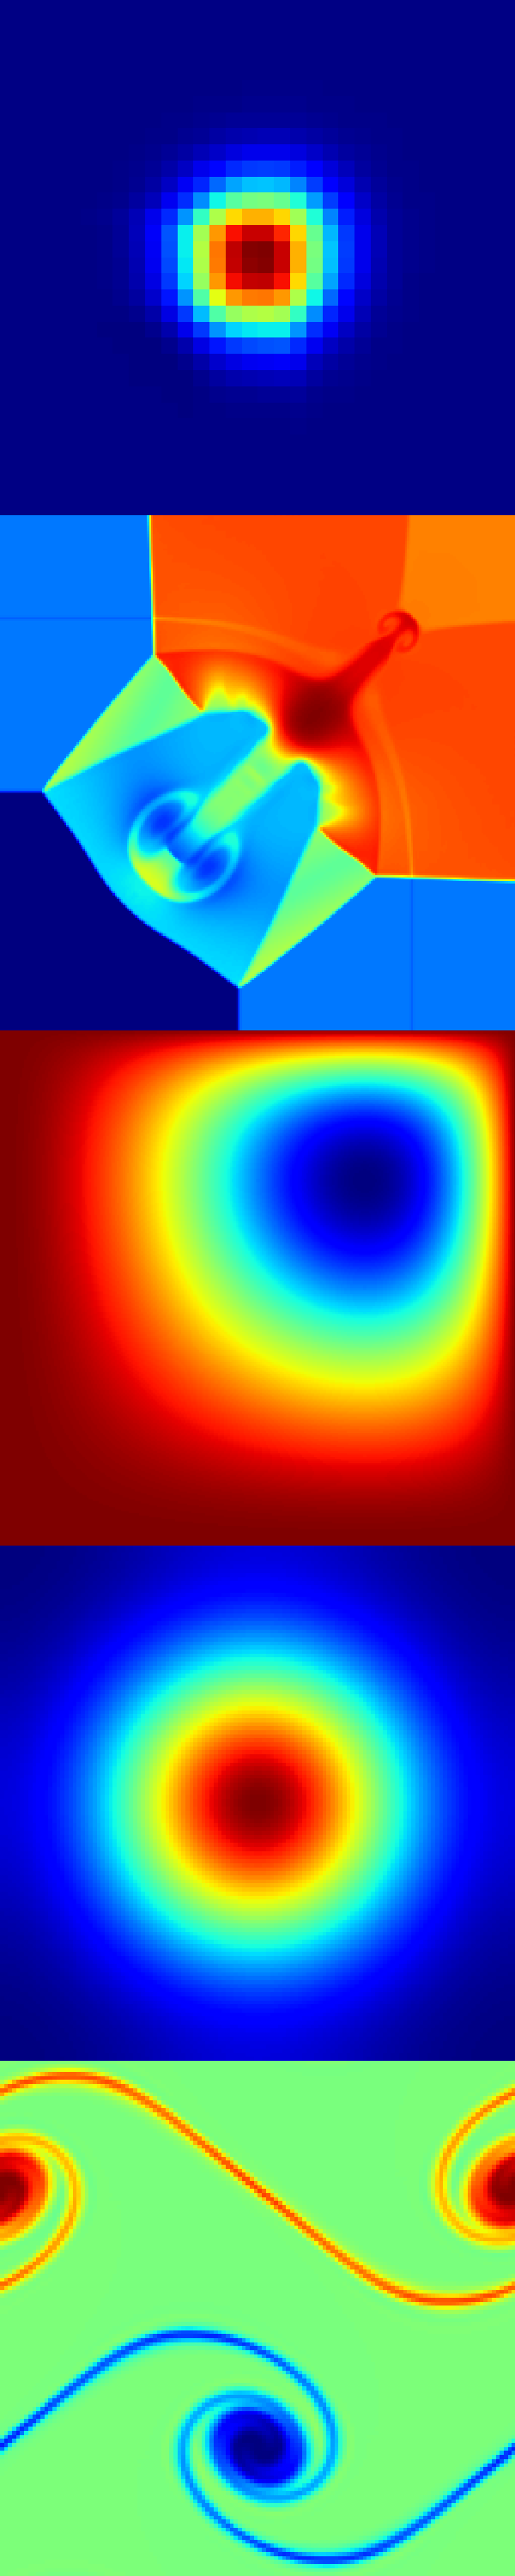
\includegraphics[width=\paperwidth,height=\paperheight,%
keepaspectratio]{images/cover.png}%
\vfill
}}}


\usepackage[many]{tcolorbox}

\newtcolorbox{mybox}[1][]{
    width=\textwidth,
    arc=0mm,
%    auto outer arc,
    boxsep=0cm,
    toprule=1pt,
    leftrule=1pt,
    bottomrule=1pt,
    rightrule=1pt,
    colframe=black,
    colback=white,
    fontupper=\centering\fontsize{40pt}{40pt}\sffamily,
    breakable,
    nobeforeafter,
    enhanced jigsaw,
    opacityframe=1.0,
    opacityback=0.7
}


\pdfpageattr{/Group <</S /Transparency /I true /CS /DeviceRGB>>}

\newcommand{\imag}{\mathsf{i}}


\begin{document}

\AddToShipoutPicture*{\BackgroundPic}

\frontmatter

\begin{titlepage}

\ \\[3.0in]
\begin{center}
%% \HRule\\[0.5em]
%% {\Huge \textsf{{
%% Lecture Notes on\\[0.1em]
%% Computational Hydrodynamics\\[0.3em]
%% for Astrophysics}}
%% }
%% \HRule
%% \\[2em]

%% {\Large \sf Michael Zingale} \\ {\sf Stony Brook University}

\begin{mybox}[]
\vskip 3mm
{Computational Hydrodynamics \\[-0.75em]
for Astrophysics\\[0.5em]}
{\Large Michael Zingale\\[-1.75em]}
{\large part of the Open Astrophysics Bookshelf}
\end{mybox}
\end{center}

\vfill

\begin{flushright}
\today
\end{flushright}

\end{titlepage}

\pagestyle{plain}

\null \vfill

\noindent \ccCopy\ 2013, 2014, 2015, 2016 Michael Zingale \\
\noindent document git version: \input git_info.tex $\ldots$

\noindent the source for these notes are available online (via \git):\\
\url{https://github.com/Open-Astrophysics-Bookshelf/numerical_exercises}

\noindent \ccbyncsa \\
\noindent This work is licensed under the Creative Commons
Attribution-NonCommercial-ShareAlike 4.0 International (CC BY-NC-SA
4.0) license.


\clearpage


\shorttoc{Chapter Listing}{0}

\clearpage


\setcounter{tocdepth}{2}
\tableofcontents

\clearpage

\listoffigures
\addcontentsline{toc}{chapter}{list of figures}

\clearpage

\listofexercise
\addcontentsline{toc}{chapter}{list of exercises}

\clearpage

\chapter*{preface}
\chaptermark{preface}
\addcontentsline{toc}{chapter}{preface}

\input preface/preface.tex

\clearpage

\pagestyle{headings}

\renewcommand{\chaptermark}[1]{%
\markboth{\chaptername
\ \thechapter.\ #1}{}}

\renewcommand{\sectionmark}[1]{\markright{\thesection---#1}}

% put the git hash on the first page of each chapter -- see section
% 7 of the fancyhdr docs to see how to override the plain
% style
\fancypagestyle{plain}{%
\fancyhf{} % clear all header and footer fields
\fancyfoot[C]{\thepage} % except the center
\fancyfoot[L]{\scriptsize git version: \input git_info.tex $\ldots$}
\renewcommand{\headrulewidth}{0pt}
\renewcommand{\footrulewidth}{0pt}}


\mainmatter

\part{Basics}

\chapter{Simulation Overview}

\input intro/intro.tex

\ifdefined\debugmode
\chapter{Classification of PDEs}

\input pde-classes/pde-classes.tex
\fi

%\addtocontents{exc}{\protect\addvspace{10pt}}%
\chapter{Finite-Volume Grids}

\input finite-volume/finite-volume.tex

\part{Advection and Hydrodynamics}

%\addtocontents{exc}{\protect\addvspace{10pt}}%
\chapter{Advection}

\input advection/advection.tex

%\addtocontents{exc}{\protect\addvspace{10pt}}%
\chapter{Burgers' Equation}

\input burgers/burgers.tex

%\addtocontents{exc}{\protect\addvspace{10pt}}%
\chapter{Euler Equations: Theory}

\input Euler/Euler-theory.tex


\chapter{Euler Equations: Numerical Methods}

\input Euler/Euler-methods.tex


\ifdefined\debugmode
\chapter{Hydrodynamics Test Problems}

\input hydro-test-problems/hydro-test-problems.tex


\chapter{Instabilities and Turbulence}

\input instabilities/instabilities.tex

\fi

\chapter{Planning a Simulation}

\input simulations/simulations.tex




\part{Elliptic, Parabolic Problems, and Mixed-Type Problems}

%\addtocontents{exc}{\protect\addvspace{10pt}}%
\chapter{Elliptic Equations and Multigrid}

\input multigrid/multigrid.tex

%\addtocontents{exc}{\protect\addvspace{10pt}}%
\chapter{Diffusion}

\input diffusion/diffusion.tex

%\addtocontents{exc}{\protect\addvspace{10pt}}%
\chapter{Multiphysics Applications}

\input multiphysics/multiphysics.tex


\part{Low Speed Hydrodynamics}

%\addtocontents{exc}{\protect\addvspace{10pt}}%
\chapter{Incompressible Flow and Projection Methods}

\input incompressible/incompressible.tex

\chapter{Low Mach Number Methods}

\input low_mach/low_mach.tex

\ifdefined\debugmode
\chapter{Radiation Hydrodynamics}

\input radiation/radiation.tex
\fi

%\part{Appendices}

\appendix

\chapter{Using \hydroex}

\input hydro_examples/hydro_examples.tex

\chapter{Using \pyro}

\input pyro/pyro.tex

%% \chapter{Software Engineering Practices}

%% \input software-engineering/software-engineering.tex

\backmatter

\addcontentsline{toc}{chapter}{References}
\bibliographystyle{plain}
\bibliography{refs}

\end{document}
